\subsubsection{UC8 - Gestione Beni Venduti}
\begin{figure}[h]
	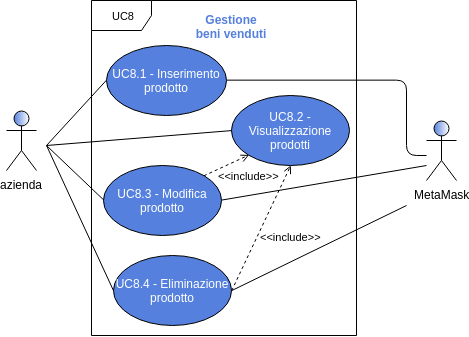
\includegraphics[width=10cm]{res/images/UC8-Generale.png}
	\centering
	\caption{UC8 - Operazioni per la gestione dei beni venduti}
\end{figure}
\begin{itemize}
	\item \textbf{Attori Primari}: azienda;
	\item \textbf{Attori Secondari}: MetaMask\glo;
	\item \textbf{Descrizione}: le aziende hanno la possibilità di gestire i beni venduti sulla piattaforma;
	\item \textbf{Scenario principale}: l'azienda accede alla pagina per la gestione dei prodotti/servizi venduti e può:
	\begin{itemize}
		\item inserire un nuovo prodotto/servizio da vendere [UC8.1];
		\item visualizzare i propri prodotti attualmente in vendita [UC8.2];
		\item modificare un prodotto/servizio già presente nella piattaforma [UC8.3];
		\item rimuovere un prodotto/servizio presente [UC8.4]; 
	\end{itemize}
	\item \textbf{Precondizione}: il sistema ha identificato l'utente come azienda, l'azienda ha espresso la volontà di gestire i propri prodotti/servizi;
	\item \textbf{Postcondizione}: il sistema fornisce all'azienda le operazioni che possono essere svolte sui propri prodotti.	
\end{itemize}

\subsubsection{UC8.1 - Inserimento prodotto}
\begin{figure}[H]
	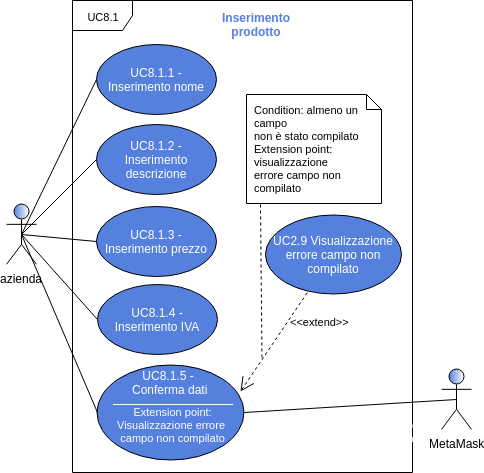
\includegraphics[width=10cm]{res/images/UC8-Inserimento.png}
	\centering
	\caption{UC8.1 - Inserimento prodotto}
\end{figure}
\begin{itemize}
	\item \textbf{Attori Primari}: azienda;
	\item \textbf{Attori Secondari}: MetaMask\glo;
	\item \textbf{Descrizione}: le aziende possono inserire dei nuovi prodotti nella piattaforma;
	\item \textbf{Scenario principale}: l'azienda accede alla pagina per inserire un nuovo prodotto e deve:
	\begin{itemize}
		\item inserire il nome del prodotto/servizio [UC8.1.1];
		\item inserire la descrizione del prodotto/servizio [UC8.1.2];
		\item inserire il prezzo netto unitario del prodotto/servizio [UC8.1.3];
		\item inserire la quantità disponibile del prodotto/servizio [UC8.1.4];
		\item confermare i dati inseriti [UC8.1.5];
		\item inserire l'IVA del prodotto/servizio [UC8.1.6].
	\end{itemize}
	\item \textbf{Precondizione}: il sistema ha identificato l'utente come azienda, l'azienda ha espresso la volontà di inserire un nuovo prodotto/servizio;
	\item \textbf{Postcondizione}: l'azienda ha inserito correttamente i dati relativi al nuovo prodotto ed è riuscita ad inserire il nuovo prodotto/servizio sulla piattaforma.	
\end{itemize}
\subsubsection{UC8.1.1 - Inserimento nome}
\begin{itemize}
	\item \textbf{Attori Primari}: azienda;
	\item \textbf{Descrizione}: al fine di portare a termine il processo di inserimento di un nuovo prodotto l'utente deve inserire il nome del prodotto, campo ritenuto obbligatorio;
	\item \textbf{Scenario principale}: l'utente compila il campo relativo al nome del nuovo prodotto/servizio da inserire;
	\item \textbf{Precondizione}: il sistema ha reso disponibile il form per l'inserimento di un nuovo prodotto/servizio, in particolare è presente il campo per l'inserimento del nome;
	\item \textbf{Postcondizione}: l'utente ha compilato il campo relativo al nome del nuovo prodotto da inserire.
\end{itemize}
\subsubsection{UC8.1.2 - Inserimento descrizione}
\begin{itemize}
	\item \textbf{Attori Primari}: azienda;
	\item \textbf{Descrizione}: al fine di portare a termine il processo di inserimento di un nuovo prodotto l'utente deve inserire la descrizione del prodotto, campo ritenuto obbligatorio;
	\item \textbf{Scenario principale}: l'utente compila il campo relativo alla descrizione del nuovo prodotto/servizio da inserire;
	\item \textbf{Precondizione}: il sistema ha reso disponibile il form per l'inserimento di un nuovo prodotto/servizio, in particolare è presente il campo per l'inserimento della descrizione;
	\item \textbf{Postcondizione}: l'utente ha compilato il campo relativo alla descrizione del nuovo prodotto da inserire.
\end{itemize}
\subsubsection{UC8.1.3 - Inserimento prezzo netto}
\begin{itemize}
	\item \textbf{Attori Primari}: azienda;
	\item \textbf{Descrizione}: al fine di portare a termine il processo di inserimento di un nuovo prodotto l'utente deve inserire il prezzo netto unitario del prodotto, campo ritenuto obbligatorio;
	\item \textbf{Scenario principale}: l'utente compila il campo relativo al prezzo del nuovo prodotto/servizio da inserire;
	\item \textbf{Precondizione}: il sistema ha reso disponibile il form per l'inserimento di un nuovo prodotto/servizio, in particolare è presente il campo per l'inserimento del prezzo;
	\item \textbf{Postcondizione}: l'utente ha compilato il campo relativo al prezzo del nuovo prodotto da inserire.
\end{itemize}
\subsubsection{UC8.1.4 - Inserimento quantità}
\begin{itemize}
	\item \textbf{Attori Primari}: azienda;
	\item \textbf{Descrizione}: al fine di portare a termine il processo di inserimento di un nuovo prodotto l'utente deve inserire il numero di pezzi disponibili del prodotto, campo ritenuto obbligatorio;
	\item \textbf{Scenario principale}: l'utente compila il campo relativo al numero di pezzi del nuovo prodotto/servizio da inserire;
	\item \textbf{Precondizione}: il sistema ha reso disponibile il form per l'inserimento di un nuovo prodotto/servizio, in particolare è presente il campo per l'inserimento alla quantità di pezzi;
	\item \textbf{Postcondizione}: l'utente ha compilato il campo relativo alla quantità di pezzi del nuovo prodotto da inserire.
\end{itemize}
\subsubsection{UC8.1.5 - Conferma dati}
\begin{itemize}
	\item \textbf{Attori Primari}: azienda;
	\item \textbf{Attori Primari}: MetaMask\glo;
	\item \textbf{Descrizione}: al fine di portare a termine il processo di registrazione l'utente deve confermare i dati inseriti tramite l'approvazione della transazione, che verrà eseguita attraverso il plugin MetaMask\glo;
	\item \textbf{Scenario principale}: l'utente preme il pulsante di conferma dei dati inseriti e valida la transazione con MetaMask\glo;
	\item \textbf{Estensioni}:
	\begin{itemize}
		\item \textbf{UC2.9}: l'utente tenta di confermare i dati senza aver compilato tutti i campi richiesti;
	\end{itemize}
	\item \textbf{Precondizione}: il sistema ha reso disponibile il form per l'inserimento dei dati riguardanti il nuovo prodotto, l'utente ha compilato tutti i campi ed ha premuto il pulsante per la conferma.
	\item \textbf{Postcondizione}: il nuovo prodotto è stato inserito nella piattaforma e l'utente ottiene la conferma della riuscita dell'operazione.
\end{itemize}
\subsubsection{UC8.1.6 - Inserimento IVA}
\begin{itemize}
	\item \textbf{Attori Primari}: azienda;
	\item \textbf{Descrizione}: al fine di portare a termine il processo di inserimento di un nuovo prodotto l'utente deve inserire la percentuale di IVA;
	\item \textbf{Scenario principale}: l'utente compila il campo relativo all'IVA del nuovo prodotto/servizio da inserire;
	\item \textbf{Precondizione}: il sistema ha reso disponibile il form per l'inserimento di un nuovo prodotto/servizio, in particolare è presente il campo per l'inserimento dell'IVA;
	\item \textbf{Postcondizione}: l'utente ha compilato il campo relativo all'IVA del nuovo prodotto da inserire.
\end{itemize}
\subsubsection{UC8.2 - Visualizzazione prodotto}
\begin{figure}[h]
	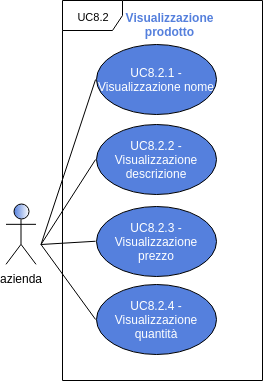
\includegraphics[width=6cm]{res/images/UC8-Visualizzazione.png}
	\centering
	\caption{UC8.2 - Visualizzazione prodotto}
\end{figure}
\begin{itemize}
	\item \textbf{Attori Primari}: azienda;
	\item \textbf{Descrizione}: le aziende possono visualizzare i loro prodotti inseriti nella piattaforma;
	\item \textbf{Scenario principale}: l'azienda accede alla pagina per visualizzare i loro prodotti. Per ogni prodotto potrà: 
	\begin{itemize}
		\item visualizzare il nome [UC8.2.1];
		\item visualizzare la descrizione [UC8.2.2];
		\item visualizzare il prezzo [UC8.2.3];
		\item visualizzare la quantità [UC8.2.4];
	\end{itemize}
	\item \textbf{Precondizione}: il sistema ha identificato l'utente come azienda, l'azienda ha espresso la volontà di visualizzare i propri prodotti inseriti nella piattaforma;
	\item \textbf{Postcondizione}: l'azienda ha ottenuto la lista dei propri prodotti assieme alle operazioni eseguibili su di essi.	
\end{itemize}
\subsubsection{UC8.2.1 - Visualizzazione nome}
\begin{itemize}
	\item \textbf{Attori Primari}: azienda;
	\item \textbf{Descrizione}: l'azienda visualizza il nome del bene o del servizio;
	\item \textbf{Scenario principale}: l'utente visualizza le informazioni relative ai propri prodotti/servizi;
	\item \textbf{Precondizione}: l'utente ha espresso la volontà di visualizzare i propri prodotti/servizi;
	\item \textbf{Postcondizione}: l'utente può visualizzare il nome del prodotto.
\end{itemize}
\subsubsection{UC8.2.2 - Visualizzazione quantità}
\begin{itemize}
	\item \textbf{Attori Primari}: azienda;
	\item \textbf{Descrizione}: l'azienda visualizza la quantità rimanente del bene o del servizio;
	\item \textbf{Scenario principale}: l'utente visualizza le informazioni relative ai propri prodotti/servizi;
	\item \textbf{Precondizione}: l'utente ha espresso la volontà di visualizzare i propri prodotti/servizi;
	\item \textbf{Postcondizione}: l'utente può visualizzare la quantità rimanente di ciascuno dei prodotti.
\end{itemize}
\subsubsection{UC8.2.3 - Visualizzazione prezzo}
\begin{itemize}
	\item \textbf{Attori Primari}: azienda;
	\item \textbf{Descrizione}: l'azienda visualizza il prezzo del bene o del servizio;
	\item \textbf{Scenario principale}: l'utente visualizza le informazioni relative ai propri prodotti/servizi;
	\item \textbf{Precondizione}: l'utente ha espresso la volontà di visualizzare i propri prodotti/servizi;
	\item \textbf{Postcondizione}: l'utente può visualizzare il prezzo del prodotto.
\end{itemize}
\subsubsection{UC8.2.4 - Visualizzazione descrizione}
\begin{itemize}
	\item \textbf{Attori Primari}: azienda;
	\item \textbf{Descrizione}: l'azienda visualizza la descrizione del bene o del servizio;
	\item \textbf{Scenario principale}: l'utente visualizza le informazioni relative ai propri prodotti/servizi;
	\item \textbf{Precondizione}: l'utente ha espresso la volontà di visualizzare i propri prodotti/servizi;
	\item \textbf{Postcondizione}: l'utente può visualizzare la descrizione del prodotto.
\end{itemize}

\subsubsection{UC8.3 - Modifica prodotto}
\begin{figure}[H]
	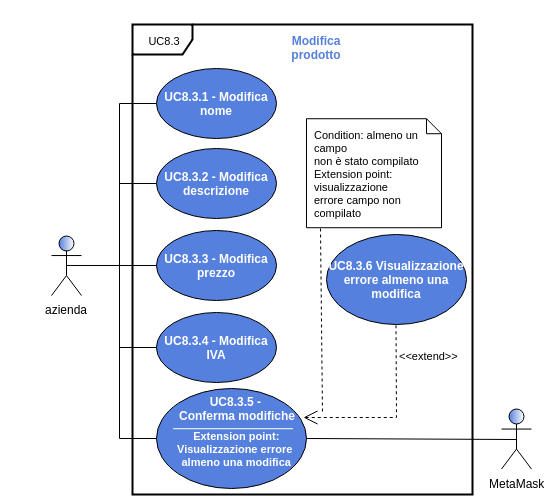
\includegraphics[width=10cm]{res/images/UC8-Modifica.png}
	\centering
	\caption{UC8.3 - Modifica prodotto}
\end{figure}
\begin{itemize}
	\item \textbf{Attori Primari}: azienda;
	\item \textbf{Attori Secondari}: MetaMask\glo;
	\item \textbf{Descrizione}: le aziende possono modificare i loro prodotti inseriti nella piattaforma;
	\item \textbf{Scenario principale}: l'azienda accede alla modifica di un prodotto attraverso l'apposito pulsante mostrato assieme alle informazioni riguardanti l'oggetto stesso[UC8.2]. Per ogni prodotto potrà: 
	\begin{itemize}
		\item modificarne il nome [UC8.3.1];
		\item modificarne la descrizione [UC8.3.2];
		\item modificarne il prezzo [UC8.3.3];
		\item modificarne la quantità [UC8.3.4];
	\end{itemize}
	Dunque dovrà confermare l'operazione attraverso l'utilizzo di MetaMask\glo.
	\item \textbf{Inclusione}:
	\begin{itemize}
		\item \textbf{UC8.2}: per poter modificare i prodotti l'azienda deve prima individuarli nella lista dei propri prodotti;
	\end{itemize}
	\item \textbf{Precondizione}: il sistema ha identificato l'utente come azienda, l'azienda ha espresso la volontà modificare un prodotto;
	\item \textbf{Postcondizione}: l'azienda ha modificato le caratteristiche del prodotto ed ha ottenuto un messaggio che conferma il successo dell'operazione.	
\end{itemize}

\subsubsection{UC8.3.1 - Modifica nome}
\begin{itemize}
	\item \textbf{Attori Primari}: azienda;
	\item \textbf{Descrizione}: l'azienda inserisce nell'apposito campo il nuovo nome del prodotto/servizio;
	\item \textbf{Scenario principale}: l'utente visualizza il vecchio nome con affianco un campo dati per inserire il nuovo nome, ed inserisce il nuovo valore;
	\item \textbf{Precondizione}: l'utente ha espresso la volontà di modificare i dati di un prodotto/servizio;
	\item \textbf{Postcondizione}: l'utente ha inserito il nuovo nome nel campo dedicato del form.
\end{itemize}

\subsubsection{UC8.3.2 - Modifica descrizione}
\begin{itemize}
	\item \textbf{Attori Primari}: azienda;
	\item \textbf{Descrizione}: l'azienda inserisce nell'apposito campo la nuova descrizione del prodotto/servizio;
	\item \textbf{Scenario principale}: l'utente visualizza la vecchia descrizione con affianco un campo dati per inserire la nuova descrizione, ed inserisce il nuovo valore;
	\item \textbf{Precondizione}: l'utente ha espresso la volontà di modificare i dati di un prodotto/servizio;
	\item \textbf{Postcondizione}: l'utente ha inserito la nuova descrizione nel campo dedicato del form.
\end{itemize}

\subsubsection{UC8.3.3 - Modifica prezzo}
\begin{itemize}
	\item \textbf{Attori Primari}: azienda;
	\item \textbf{Descrizione}: l'azienda inserisce nell'apposito campo il nuovo prezzo del prodotto/servizio;
	\item \textbf{Scenario principale}: l'utente visualizza il vecchio prezzo con affianco un campo dati per inserire il nuovo prezzo, ed inserisce il nuovo valore;
	\item \textbf{Precondizione}: l'utente ha espresso la volontà di modificare i dati di un prodotto/servizio;
	\item \textbf{Postcondizione}: l'utente ha inserito il nuovo prezzo nel campo dedicato del form.
\end{itemize}

\subsubsection{UC8.3.4 - Modifica quantità}
\begin{itemize}
	\item \textbf{Attori Primari}: azienda;
	\item \textbf{Descrizione}: l'azienda inserisce nell'apposito campo la nuova quantità del prodotto/servizio;
	\item \textbf{Scenario principale}: l'utente visualizza la vecchia quantità con affianco un campo dati per inserire la nuova quantità, ed inserisce il nuovo valore;
	\item \textbf{Precondizione}: l'utente ha espresso la volontà di modificare i dati di un prodotto/servizio;
	\item \textbf{Postcondizione}: l'utente ha inserito la nuova quantità nel campo dedicato del form.
\end{itemize}

\subsubsection{UC8.3.5 - Conferma modifiche}
\begin{itemize}
	\item \textbf{Attori Primari}: azienda;
	\item \textbf{Attori Primari}: MetaMask\glo;
	\item \textbf{Descrizione}: al fine di portare a termine il processo di modifica dei dati di un prodotto/servizio, l'utente deve confermare i dati inseriti tramite l'approvazione della transazione, che verrà eseguita attraverso il plugin MetaMask\glo;
	\item \textbf{Scenario principale}: l'utente preme il pulsante di conferma dei dati inseriti e valida l'operazione con MetaMask\glo;
	\item \textbf{Estensioni}:
	\begin{itemize}
		\item \textbf{UC8.3.6}: l'utente tenta di confermare i dati senza aver compilato almeno uno dei campi;
	\end{itemize}
	\item \textbf{Precondizione}: il sistema ha reso disponibile il form per la modifica dei dati riguardanti un prodotto. L'utente ha compilato almeno un campo ed ha premuto il pulsante per la conferma.
	\item \textbf{Postcondizione}: il prodotto è stato aggiornato con i nuovi dati e l'utente ottiene la conferma della riuscita dell'operazione.
\end{itemize}

\subsubsection{UC8.3.6 - Visualizzazione errore almeno una modifica}
\begin{itemize}
	\item \textbf{Attori Primari}: azienda;
	\item \textbf{Descrizione}:
	l'utente visualizza un messaggio di errore relativo al fatto nessuno dei campi per la modifica è stato compilato, e che quindi non è possibile attuare alcuna modifica;
	\item \textbf{Scenario principale}: l'utente tenta di confermare ed inviare le modifiche ai dati senza aver compilato almeno uno dei campi del form;
	\item \textbf{Precondizione}: il sistema permette all'utente di compilare il form per le modifiche. L'utente ha premuto il pulsante di conferma senza aver modificato almeno uno dei campi; 
	\item \textbf{Postcondizione}:
	l'utente è consapevole che per effettuare una modifica, almeno uno dei dati presenti deve essere stato modificato, compilando almeno uno dei campi del form.
\end{itemize}

\subsubsection{UC8.4 - Eliminazione prodotto}
\begin{itemize}
	\item \textbf{Attori Primari}: azienda;
	\item \textbf{Attori Primari}: MetaMask\glo;
	\item \textbf{Descrizione}:
	l'utente elimina uno dei propri prodotti/servizi presenti sulla piattaforma;
	\item \textbf{Scenario principale}: l'utente clicca sul pulsante di eliminazione prodotto, mostrato assieme alle informazioni riguardanti l'oggetto stesso [UC8.2]. Dunque dovrà confermare l'operazione attraverso l'utilizzo di MetaMask\glo;
	\item \textbf{Inclusione}:
	\begin{itemize}
		\item \textbf{UC8.2}: per poter eliminare i prodotti l'azienda deve prima individuarli nella lista dei propri prodotti;
	\end{itemize}
	\item \textbf{Precondizione}: il sistema ha identificato l'utente come azienda, l'azienda ha espresso la volontà eliminare un prodotto;
	\item \textbf{Postcondizione}: l'azienda ha eliminato il prodotto ed ha ottenuto un messaggio che conferma il successo dell'operazione.
\end{itemize}


